\documentclass[12pt, a4paper]{paper}
\usepackage{graphicx}
\usepackage{float}
\usepackage{amsmath,amsfonts,amsthm}

\newcommand{\transitionProb}[0]{$P_{ss'}^{a}$}
\newcommand{\reward}[0]{$R_{s}^{a}$}
\newcommand{\policy}[0]{$\pi$}
\newcommand{\statevalfunction}[0]{$v_{\pi}(s) = \mathbb{E} [G_{t} | S_{t} = s]$}
\newcommand{\statereturn}[0]{$G_{t} = R_{t+1} + \gamma R_{t+2} +...+ \gamma^{T-1} R_{T}$}

\title{Reinforcement Learning \\ Model Free Prediction}

\author{ Lu Hong }

\date{\today}

\begin{document}

\maketitle	
% ----------------------------------------------
% 
% ----------------------------------------------

% ----------------------------------------------
% CONTENTS
% ----------------------------------------------


% ----------------------------------------------
% INTRODUCTION
% ----------------------------------------------

\section{Introduction}
In Dynamic Programming Lecture, we can solve a MDP using given model using DP method, by iteration to achieve the optimal value function.
There exists two methods: policy gradient and value gradient.

In this chapter, we don't know the model. It means we don't know \transitionProb and \reward, in order to learn from environment, 
agent has to interact with the environment, generating several episodes. This lecture illustrate MC method, and extends to the TD 
algorithm, along with TD($\lambda$) method.


\begin{figure}[h]
	\begin{center}
		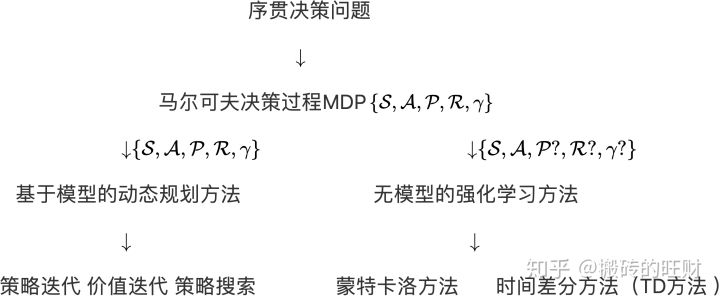
\includegraphics[width = \linewidth]{v2-52171db8d68b627b78282004c1c564f9_hd.jpg}				
	\end{center}
\end{figure}

% ----------------------------------------------
% MC
% ----------------------------------------------
\section{Monte-Carlo Reinforcement Learning}

\subsection{Overview}
\begin{itemize}
	\item learn directly from \textit{episodes of experience}
	\item model-free: no knowledge of MDP transitions / rewards
	\item learns from complete episodes: \textbf{no bootsrapping}
	\item use the simplest possible idea: value = mean return
	\item all episodes must be terminated
\end{itemize}

\subsection{Monte-Carlo Policy Evaluation}
Given a \policy, an episode can be represented as follows:

$S_{1}, A_{1}, R_{2}, S_{2}, A_{2}, ..., S_{t}, A_{t}, R_{t+1}, ..., S_{T} ~ \pi$

Recall that \statevalfunction, where \statereturn

Now, in MC method, if the state $s$ appears multiple times in one episode, like $t_{1}, t_{2}$, how can we evaluate the policy?
\subsubsection{First-Visit Monte-Carlo Policy Evaluation}
\begin{figure}[h]
	\begin{center}
		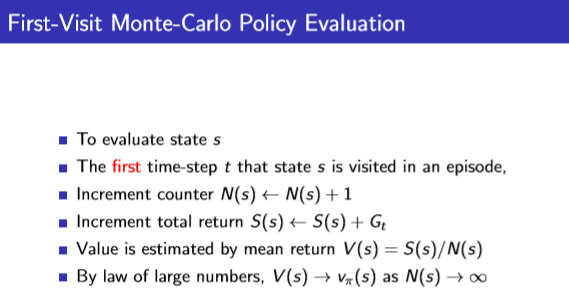
\includegraphics[width = \linewidth]{firstVisit.png}
	\end{center}
\end{figure}

\textbf{Every sampled trajectory is i.i.d.}

\subsubsection{Every-Visit Monte-Carlo Policy Evaluation}
\begin{figure}[h]
	\begin{center}
		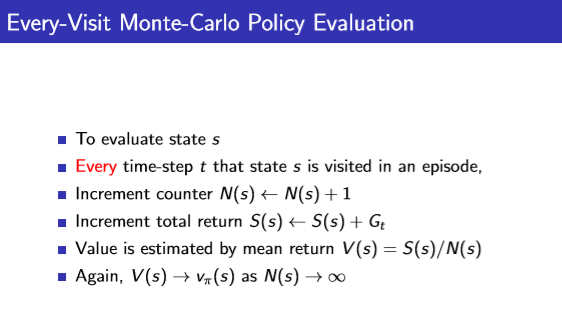
\includegraphics[width = \linewidth]{everyVisit.png}
	\end{center}
\end{figure}

\subsection{Incremental Monte-Carlo Updates}

We compute the mean value incrementally, for each state $S_{t}$ with return $G_{t}$
\begin{equation*}
	\begin{aligned}[l]
		N(S_{t}) &\leftarrow N(S_{t}) + 1 \\
		V(S_{t}) &\leftarrow V(S_{t}) + \frac{1}{N(S_{t})}(G_{t} - V(S_{t}))
	\end{aligned}
\end{equation*}

In non-stationary problems, it can be useful to track a running mean, i.e. forget old episodes. From my perspective,
it means forget $N(S_{t})$ in mathmatics, turning $\alpha$ into a parameter likes learning rate.
\begin{equation*}
	\begin{aligned}
		V(S_{t}) &\leftarrow V(S_{t}) + \alpha (G_{t} - V(S_{t}))
	\end{aligned}
\end{equation*}

Apparently, MC method requires episodes to be terminated and it also requires much time to 

% ----------------------------------------------
% TD
% ----------------------------------------------

\section{TD Learning \\ Temporal-Difference Learning}
\begin{figure}[h]
	\begin{center}
		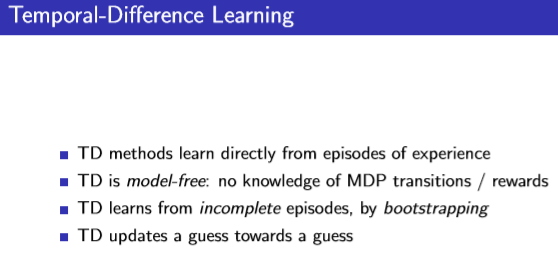
\includegraphics[width=\linewidth]{TDlearning.png}
	\end{center}
\end{figure}

Here, bootsrapping means using TD-target to replace $G_{t}$ which in TD(0), TD target = $R_{t+1} + \gamma V(S_{t+1})$

\begin{figure}[h]
	\begin{center}
		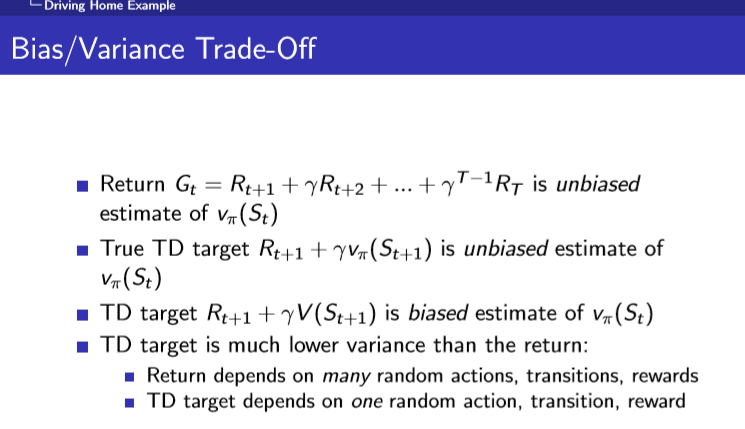
\includegraphics[width=\linewidth]{BiasVarianceTradeoff.png}
	\end{center}
\end{figure}
Where MC has high variance, zero bias. TD has low variance, some bias.

% ----------------------------------------------
% Batch MC and TD
% ----------------------------------------------
\subsection{Batch MC and TD}

We have to use limited trials to evaluate the policy, other than infinite trials.
So using batch method can make us generate limited experience and evaluate the policy.

For example, in k episodes
\begin{equation*}
	\begin{aligned}
		&s_{1}^{1}, a_{1}^{1}, r_{2}^{1}, ..., s_{T_{1}}^{1} \\ 
		&...\\
		&s_{1}^{K}, a_{1}^{K}, r_{2}^{K}, ..., s_{T_{K}}^{K}	
	\end{aligned}
\end{equation*}

David Silver uses AB example to illustrate it.
\begin{figure}[h]
	\begin{center}
		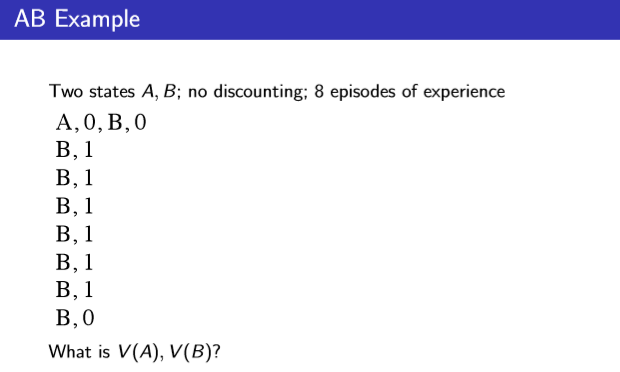
\includegraphics[width=\linewidth]{AB.png}
	\end{center}
\end{figure}

By applying MC and TD method to this problem, we can get two different value of $V(A)$

\subsection{Certainty Equivalence}
MC converges to solution with minimum mean-squared error, best fit to the observed
returns.
\begin{equation*}
	\sum_{k=1}^{K} \sum_{t=1}^{T_{k}} (G_{t}^{k} - V(s_{t}^{k}))^2
\end{equation*}

TD(0) converges to solution of \textbf{max likelihood Markov model}.
Solution to the MDP$<S, A, \hat{P}, \hat{R}, \gamma>$ that best fits the data
\begin{equation*}
	\begin{aligned}
		\hat{P}_{s,s'}^{a} &= \frac{1}{N(s,a)}\sum_{k=1}^{K} \sum_{t=1}^{T_{k}} \textbf{1}(s_{t}^{k}, a_{t}^{k},s_{t+1}^k = s, a, s')\\
		\hat{R}_{s}^{a} &= \frac{1}{N(s,a)}\sum_{k=1}^{K} \sum_{t=1}^{T_{k}} \textbf{1}(s_{t}^{k}, a_{t}^{k} = s, a)r_{t}^{k}
	\end{aligned}
\end{equation*}

\subsection{Monte-Carlo Backup}
\begin{figure}[h]
	\begin{center}
		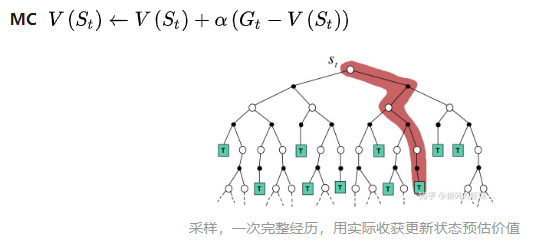
\includegraphics[width=\linewidth]{MCbackup.png}
		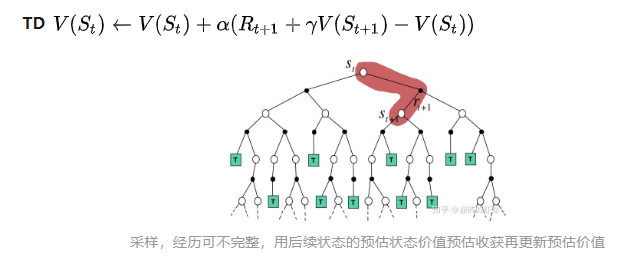
\includegraphics[width=\linewidth]{TDbackup.png}
		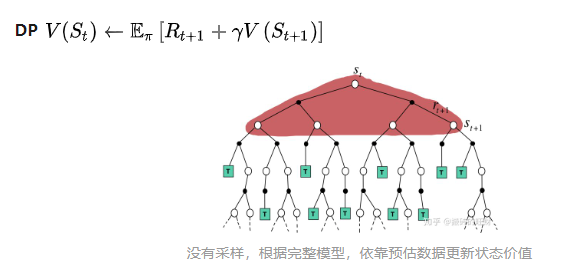
\includegraphics[width=\linewidth]{DPbackup.png}
	\end{center}
\end{figure}


% ----------------------------------------------
% TD(\lambda)
% ----------------------------------------------
\section{TD($\lambda$)}

So we use TD($\lambda$) to bridge between TD(0) and MC method, we let TD-target to 
look n-step into the future in an episode.

Now, consider n-Step return. Consider the following n-step returns for n=1,2,$\infty$:
\begin{equation*}
	\begin{aligned}
		n &= 1 (TD) \;&G_{t}^{(1)} = R_{t+1} + \gamma V(S_{t+1}) \\
		n &= 2 \;&G_{t}^{(2)} = R_{t+1} + \gamma R_{t+2} + \gamma^2 V(S_{t+2}) \\
		...\\
		n &= \infty (MC) \; &G_{t}^{(\infty)} = R_{t+1} + \gamma R_{t+2} + ... + \gamma^{T-1}R_{T}
	\end{aligned}
\end{equation*}

 So we define n-step return as 
 $$ G_{t}^{(n)} = R_{t+1} + \gamma R_{t+2} + ... + \gamma^{n-1}R_{t+n} + \gamma^{n}V(S_{t+n}) $$
 
 n-step TD learning

$$ V(S_{t}) \leftarrow V(S_{t}) + \alpha(G_{t}^{(n)} - V(S_{t}))$$

Can we efficiently combine information from all time-steps? So we introduced $\lambda-return$

\begin{itemize}
	\item The $\lambda-return$ $G_{t}^{\lambda}$ combines all n-step return $G_{t}^{(n)}$
	\item Using weight $(1-\lambda)\lambda^{n-1}$, as $G_{t}^{\lambda} = (1-\lambda) \sum_{n=1}^{\infty} \lambda^{n-1}G_{t}^{(n)}$
	\item Forward-view TD($\lambda$), as  $V(S_{t}) \leftarrow V(S_{t}) + \alpha(G_{t}^{\lambda} - V(S_{t}))$
\end{itemize}

\subsection{Back-view TD($\lambda$)}
\subsubsection{Eligibility Traces}
\begin{itemize}
	\item Frequency heuristic: assign credit to most frequent states
	\item Recency heuristic: assign credit to most recent states
	\item Eligibility traces combine both heuristics
\end{itemize}
$$ E_{0}(s) = 0 $$
$$ E_{t}(s) = \gamma \lambda E_{t-1}(s) + \textbf{1}(S_{t} = s)$$

\begin{figure}[h]
	\begin{center}
		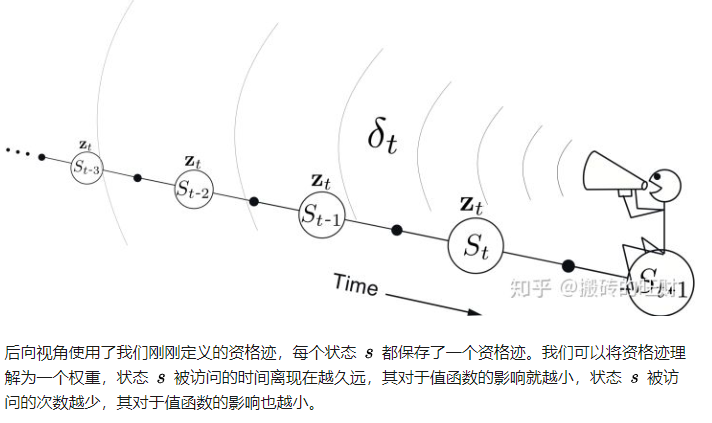
\includegraphics[width=\linewidth]{back-view.png}
	\end{center}
\end{figure}

\end{document}
